\documentclass[a4paper,12pt]{article}
\usepackage{polski}
\usepackage[utf8]{inputenc}
\usepackage[OT4]{fontenc}
\usepackage{mathtools}
\usepackage{float}
\usepackage{graphicx}
\usepackage{multirow}

\newcommand{\h}[1]{\noindent \bf #1 \rm \\ \noindent}
\newcommand{\italic}[1]{\it #1 \rm}

\begin{document}
	
\begin{center}
	\LARGE
	Struktury Danych i Złożoność Obliczeniowa \\
	\large
	ĆWICZENIA 3 
\end{center}
\vspace{1cm}	

\h{Drzewo BST:}
Drzewo poszukiwań binarnych (Binary Search Tree). Dla każdego węzła (elementu) w tym drzewie zachodzi warunek taki, że:
\begin{itemize}
	\item Wszystkie elementy lewego poddrzewa są nie większe (mniejsze lub równe) wartości węzła.
	\item Wszystkie elementy prawego poddrzewa są nie mniejsze (większe lub równe) wartości węzła.
\end{itemize}
\vspace{5mm}

\begin{figure}[H]
	\centering
	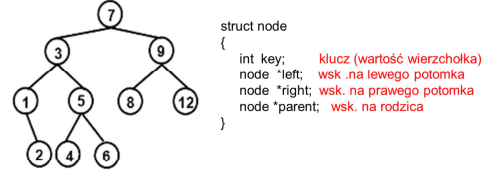
\includegraphics[width=14cm]{fig1.png}
\end{figure}

\noindent
W przeciwieństwie do kopca w drzewie BST nie ma wymogu zapełnienia wszystkich rzędów. Przez to niemożliwa jest jego tablicowa implementacja. W programie drzewo BST jest widziane tylko za pośrednictwem swojego korzenia.\\

\newpage
\h{Operacje na całości drzewa:}
Jeżeli chodzi o wykonywanie operacji na każdym wierzchołku drzewa to mamy do dyspozycji 3 podejścia (każde z nich wykorzystujące rekurencję):
\begin{itemize}
	\item \italic{preorder} - najpierw wykona się operacja dla wierzchołka, w którym jesteśmy, następnie dla kolejno lewego i prawego poddrzewa.
	\begin{figure}[H]
		\centering
		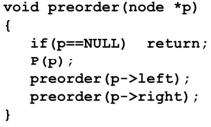
\includegraphics[width=5cm]{fig2.png}
	\end{figure}

	\item \italic{inorder} - najpierw wykona się operacja dla lewego poddrzewa, potem na aktualnego wierzchołka, potem dla prawego poddrzewa.
	\begin{figure}[H]
		\centering
		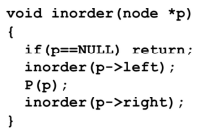
\includegraphics[width=5cm]{fig3.png}
	\end{figure}

	\item \italic{postorder} - najpierw wykonają się operacje dla lewego i prawego poddrzewa a na końcu dla aktualnego wierzchołka.
	\begin{figure}[H]
		\centering
		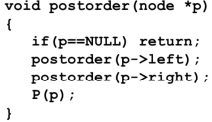
\includegraphics[width=5cm]{fig4.png}
	\end{figure}
\end{itemize}

\newpage
\h{Wyszukiwanie w BST:}
Wyszukiwanie w drzewie BST polega na wyborze odpowiedniego poddrzewa. Jeżeli wiemy, że szukana wartość jest mniejsza od wartości aktualnie rozważanego węzła, to musimy przejść do przeszukiwania jego lewego poddrzewa. Gdy jego większa, to należy przeszukać prawe poddrzewo. Wyszukiwanie kończymy, gdy odnajdziemy wartość lub, gdy dojdziemy do końca drzewa.\\

\noindent
Złożoność obliczeniowa drzewa zależy od jego stanu zapełnienia. Gdy wszystkie poziomy są zapełnione, to wyszukwiwanie ma złożoność $O(\log n)$ (przypadek optymistyczny). W przeciwnym wypadku złożoność wynosi $O(n)$. \\

\h{Znalezienie minimum/maksimum:}
Znalezienie wartości największej lub największej w drzewie BST jest dosyć proste. Najmniejszy element to ten, wysunięty najbardziej na lewo. Największy, to ten wysunięty najbardziej na prawo.\\

\h{Dodanie nowego elementu:}
Dodanie elementu zawsze sprowadza się do dodania nowego liścia do naszego drzewa. Algorytm dodawania elementu najpierw szuka dla niego rodzica, a następnie wstawia go w odpowiedniej pozycji w odniesieniu do tego rodzica (lewo/prawo). W wypadku, gdy drzewo jest puste, to nowy element staje się po prostu korzeniem.\\

\h{Następnik klucza:}
Następnik klucza $X$ to taki element, który jest większy od $X$ (znajduje się w prawym poddrzewie), ale jednocześnie będący najbliższy do $X$. Jest to po prostu minimalny element prawego poddrzewa $X$.\\

\noindent
W wypadku, gdy $X$ nie ma prawego poddrzewa (jest maksimum swojego poddrzewa), to następnikiem będzie pierwszy węzeł-rodzić, od którego nasz węzeł jest mniejszy (w którego lewym poddrzewie się znajduje).\\

\noindent
Oczywiście możliwe jest, że węzeł nie będzie mieć następnika. Dzieje się tak w sytuacji, gdy rozważany węzeł zawiera maksimum drzewa.\\

\newpage
\h{Poprzednik klucza:}
Poprzednik klucza $X$ to taki element, który jest mniejszy od $X$, ale jednocześnie jest najbliższy do $X$. Jest to po prostu maksymalny element lewego poddrzewa.\\

\noindent
W wypadku, gdy $X$ nie ma lewego poddrzewa (jest minimum swojego poddrzewa), to poprzednikiem będzie pierwszy węzeł-rodzic, od którego nasz węzeł jest większy (w którego prawym poddrzewie się znajduje).\\

\noindent
Możliwe jest, że węzeł nie będzie mieć poprzednika. Dzieje się tak w sytuacji, gdy rozważany węzeł zawiera minimum drzewa.\\

\h{Usuwanie węzła:}
Gdy węzeł jest liściem, to jego usunięcie jest trywialne. Po prostu odłączamy go od drzewa i usuwamy.\\

\noindent
Jeżeli węzeł ma jednego potomka, to po jego usunięciu na jego miejsce wstawiamy tegoż potomka.\\

\noindent
Jeżeli węzeł ma więcej potomków, to w miejsce jego wartości wstawiamy wartość jego następnika. Następnie usuwamy jego następnik.\\

\h{Rotacja w prawo:}
Operacja zmieniająca strukturę drzewa, ale nie zmieniająca wartości kluczy. Rotacja w prawo względem węzła X da efekt:
\begin{figure}[H]
	\centering
	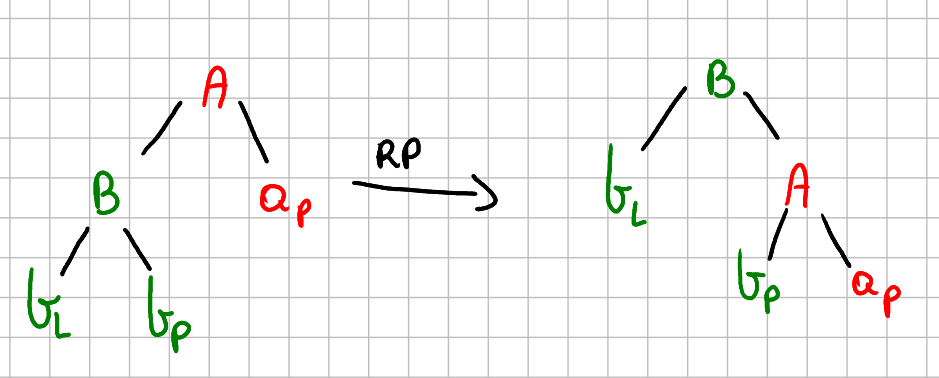
\includegraphics[width=10cm]{fig5.png}
\end{figure}

\newpage
\h{Rotacja w lewo:}
Operacja zmieniająca strukturę drzewa, ale nie zmieniająca wartości kluczy. Rotacja w lewo względem węzła X da efekt:
\begin{figure}[H]
	\centering
	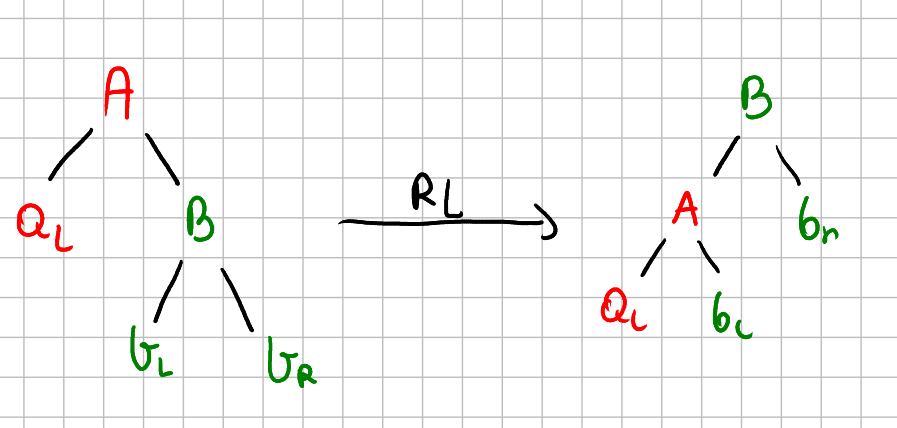
\includegraphics[width=10cm]{fig6.png}
\end{figure}

\h{Drzewo zrównoważone:}
Drzewo BTS, w którym wysokości lewego i prawego poddrzewa nie różnią się o więcej niż 1.
\begin{figure}[H]
	\centering
	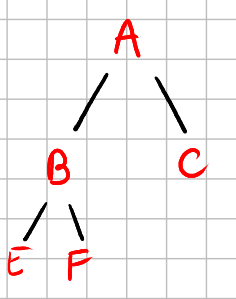
\includegraphics[width=3cm]{fig7.png}
\end{figure}

\h{Drzewo doskonale zrównoważone:}
Drzewo zrównoważone, w którym wszystkie liście znajdują się maksymalnie na dwóch poziomach.\\

\h{Algorytm równoważenia drzewa (DSW):}
Algorytm pozwala na uzyskanie zrównoważonego drzewa BST. Jest to ważne, gdyż do takiego drzewa uzyskamy najmniejszą złożoność dla algorytmu wyszukiwania. W pierwszym etapie algorytmu wykonuje się prostowanie drzewa (sprowadzenie go do postaci liniowej) poprzez szereg rotacji w prawo. W drugim etapie wykorzystuje się szereg rotacji w lewo, w celu utrzymania drzewa zrównoważonego.
\begin{figure}[H]
	\centering
	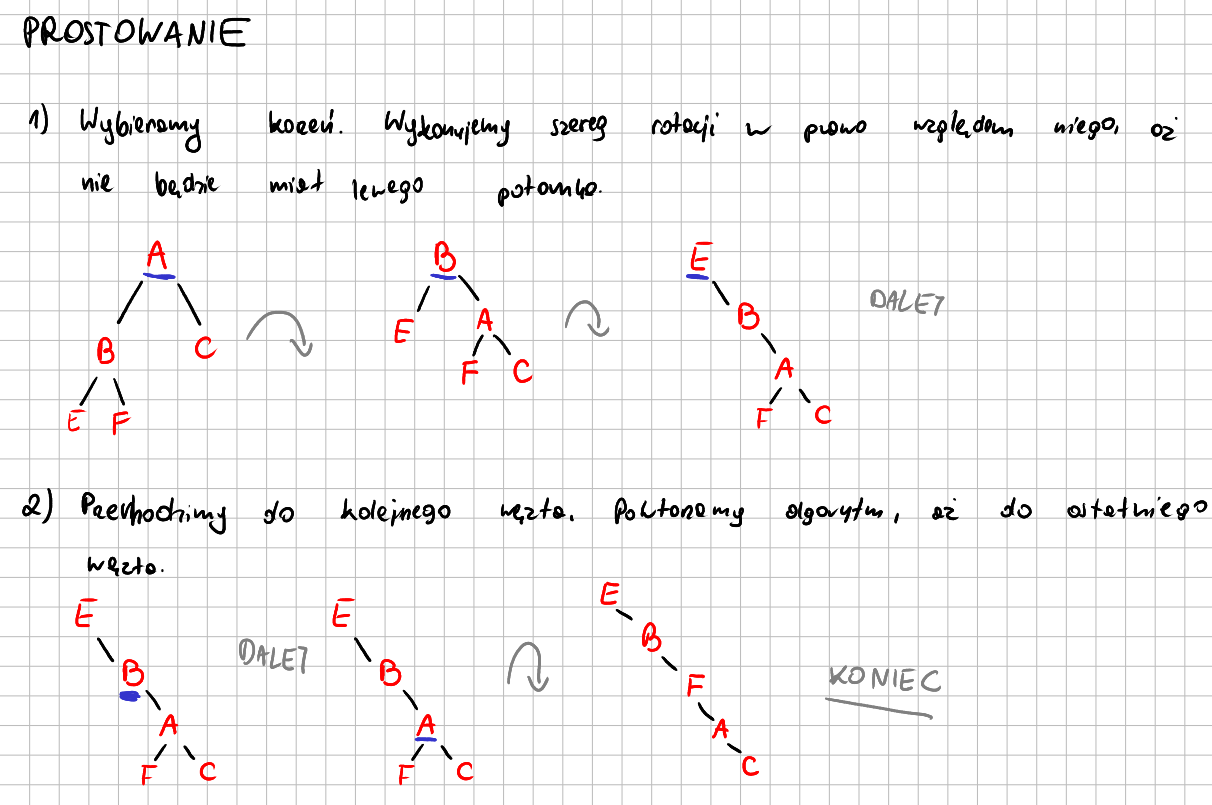
\includegraphics[width=14cm]{fig8.png}
\end{figure}
\begin{figure}[H]
	\centering
	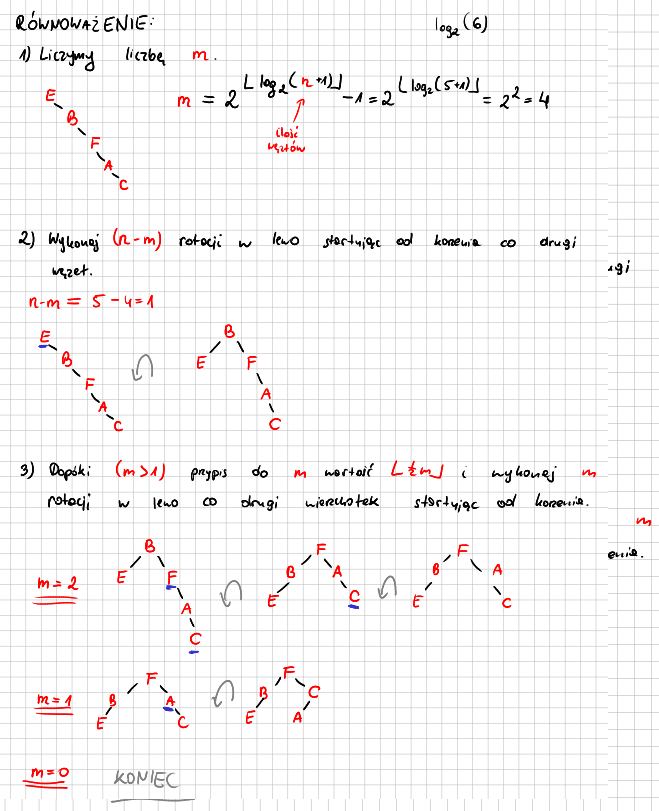
\includegraphics[width=14cm]{fig9.png}
\end{figure}

	
\end{document}